\section{Apstraktna sintaksička stabla}
\label{sec:AST}

Kako bi se k\^od pisan u nekom programskom jeziku (\emph{izvorni fajl}) preveo u k\^od koji će se izvršavati na nekoj mašini (\emph{izvršivi fajl}), prevodilac izvršava određene korake. Prvi korak je prepoznavanje gradivnih elemenata programskog jezika koji se nazivaju \emph{lekseme}, nalik na prepoznavanje reči u rečenicama govornog jezika, i raspodela leksema u grupe po funkciji (nalik na funkcije reči u govornom jeziku --- subjekti, predikati, objekti itd.). Nakon prepozavanja leksema, proverava se da li niz prepoznatih leksema ispunjava pravila odnosno \emph{sintaksu} programskog jezika, nalik na proveru da li se složene govorne rečenice sastoje od subjekta i predikta u određenom redosledu. Na kraju se proverava značenje odnosno \emph{semantika} koda, nalik na proveru da li govorne rečenice, iako sintaksno pravilne, imaju smisla. Deo prevodioca koji određuje da li je izvorni k\^od ispravno formiran u terminima leksike, sintakse i semantike se naziva \emph{prednji deo} (engl. \emph{front end}). Ukoliko je izvorni k\^od ispravan, prednji deo kreira \emph{međureprezentaciju} koda (engl. \emph{intermediate representation}, u daljem tekstu \emph{IR}) nad kojom se vrše optimizacije koda i koja se koristi za dalji proces prevođenja. Ukoliko to nije slučaj, prevođenje ne uspeva i programeru se daje poruka sa obrazloženjem zašto prevođenje nije uspelo \cite{EngineeringCompilers}.

Za potrebe ovog rada, što se procesa prevođenja tiče, dovoljno je poznavanje pomenutih procesa koje izvodi prednji deo, stoga neće biti reči o ostalim koracima u fazi prevođenja (generisanje IR, optimizovanje). Zainteresovani čitalac može više detalja pronaći u \cite{DragonBook}, \cite{EngineeringCompilers} i \cite{CompilerConstruction}. 

Pretpostavimo da želimo da prevedemo izvorni k\^od pisan u programskom jeziku C sa slike \ref{fig:CompilationProcessInit}. Primetimo da postoji greška u datom kodu --- simbol \texttt{c} koji se koristi u dodeli u liniji $7$ će biti prepoznat kao identifikator koji ne odgovara nijednoj deklarisanoj promenljivoj --- stoga ne možemo prevesti ovaj k\^od. Ovo nije greška u sintaksi --- izraz \texttt{a+c} je validan u programskom jeziku C. Problem će postati vidljiv tek nakon parsiranja izvornog koda i provere ispunjenosti sintaksih pravila, tačnije u fazi semantičke provere. Stoga se ovakve greške nazivaju \emph{semantičke greške}, dok se greške u sintaksi nazivaju \emph{sintaksne greške}.

\begin{figure}[h!]
\begin{lstlisting}
#include<stdio.h>
#define T int

int main()
{
    T a, b;
    a = a + c;        // c nije deklarisano
    printf("%d", a);
    return 0;
}
\end{lstlisting}
\caption{Primer izvornog koda sa semantičkom greškom (C).}
\label{fig:CompilationProcessInit}
\end{figure}

Pre nego što prednji kraj prevodioca dobije k\^od koji treba da prevede u međureprezentaciju, vrši se \emph{pretprocesiranje} od strane programa koji se naziva \emph{pretprocesor}. U fazi pretprocesiranja se izvode samo tekstualne operacije kao što su brisanje komentara ili zamena makroa u jezicima kao što je C. Rezultat rada pretprocesora za izvorni k\^od sa slike \ref{fig:CompilationProcessInit} se može videti na slici \ref{fig:CompilationProcessPrep}\footnote{U nekim implementacijama C standardne biblioteke, moguće je da se poziv funckije \texttt{printf} zameni pozivom funkcije \texttt{fprintf} sa ispisom na \texttt{stdout}. U standardu se propisuje da funkcije kao što je \texttt{printf} mogu biti implementirane kao makroi. Izlaz na slici \ref{fig:CompilationProcessPrep} je generisan od strane \texttt{GCC 7.4.0} po C11 standardu i ovo nije slučaj u datom okruženju.}.

\begin{figure}[h!]
\begin{lstlisting}
# 1 "<stdin>"
# 1 "<built-in>"
# 1 "<command-line>"
# 31 "<command-line>"
# 1 "/usr/include/stdc-predef.h" 1 3 4

...

extern char *ctermid (char *__s) __attribute__ ((__nothrow__ , __leaf__));
# 840 "/usr/include/stdio.h" 3 4
extern void flockfile (FILE *__stream) __attribute__ ((__nothrow__ , __leaf__));
extern int ftrylockfile (FILE *__stream) __attribute__ ((__nothrow__ , __leaf__)) ;
extern void funlockfile (FILE *__stream) __attribute__ ((__nothrow__ , __leaf__));
# 868 "/usr/include/stdio.h" 3 4
# 2 "<stdin>" 2
# 2 "<stdin>"

int main()
{
    int a, b;
    a = a + c;
    printf("%d", a);
    return 0;
}
\end{lstlisting}
\caption{Prikaz rezultata rada pretprocesora za izvorni k\^od sa slike \ref{fig:CompilationProcessInit}. Pritom, prikazano je samo par linija sa početka i kraja izlaza pretprocesora --- k\^od iznad \texttt{main} funkcije je uključen iz \texttt{stdio.h} zaglavlja.}
\label{fig:CompilationProcessPrep}
\end{figure}

U toku faze leksičke analize, kako prevodilac ne bi radio nad sirovim karakterima izvornog koda, potrebno je izvršiti transformaciju karaktera izvornog koda. Prevodilac ima u vidu elemente programskog jezika i šablone za njihovo prepoznavanje. Lekseme su one sekvence karaktera izvornog koda koje zadovoljavaju ove šablone. Lekseme se dalje razvrstavaju u kategorije, tzv. \emph{tokene} --- ključne reči, operatore, promenljive itd. Proces dobijanja tokena od izvornog koda se naziva \emph{tokenizacija}. Komponenta prednjeg dela koja vrši tokenizaciju se naziva \emph{skener} ili \emph{lekser}. Pojednostavljen primer šablona koje lekser pokušava da prepozna se mogu videti na slici \ref{fig:CLexerExample}. Primer izlaza leksera za izlaz pretprocesora sa slike \ref{fig:CompilationProcessPrep} se može videti na slici \ref{fig:CompilationProcessLex}.

\begin{figure}[h!]
\begin{lstlisting}[language={}]
Identifier 
    : IdentifierNondigit (IdentifierNondigit | Digit)*
    ;
IdentifierNondigit  
    : Nondigit
    | UniversalCharacterName
    ;
Nondigit 
    : [a-zA-Z_]
    ;
Digit 
    : [0-9]
    ;
\end{lstlisting}
\caption{Primer delimične definicije tokena za ime promenljive po C11 standardu.}
\label{fig:CLexerExample}
\end{figure}

\begin{figure}[h!]
\begin{lstlisting}[language={}]
identifier 'main'	 [LeadingSpace]	Loc=<sample.c:3:5>
l_paren '('		Loc=<sample.c:3:9>
r_paren ')'		Loc=<sample.c:3:10>
l_brace '{'	 [StartOfLine]	Loc=<sample.c:4:1>
int 'int'	 [StartOfLine] [LeadingSpace]	Loc=<sample.c:5:5>
identifier 'a'	 [LeadingSpace]	Loc=<sample.c:5:9>
comma ','		Loc=<sample.c:5:10>
identifier 'b'	 [LeadingSpace]	Loc=<sample.c:5:12>
semi ';'		Loc=<sample.c:5:13>
identifier 'a'	 [StartOfLine] [LeadingSpace]	Loc=<sample.c:6:5>
equal '='	 [LeadingSpace]	Loc=<sample.c:6:7>
identifier 'a'	 [LeadingSpace]	Loc=<sample.c:6:9>
plus '+'	 [LeadingSpace]	Loc=<sample.c:6:11>
identifier 'c'	 [LeadingSpace]	Loc=<sample.c:6:13>
semi ';'		Loc=<sample.c:6:14>
identifier 'printf'	 [StartOfLine] [LeadingSpace]	Loc=<sample.c:7:5>
l_paren '('		Loc=<sample.c:7:11>
string_literal '"%d"'		Loc=<sample.c:7:12>
comma ','		Loc=<sample.c:7:16>
identifier 'a'	 [LeadingSpace]	Loc=<sample.c:7:18>
r_paren ')'		Loc=<sample.c:7:19>
semi ';'		Loc=<sample.c:7:20>
return 'return'	 [StartOfLine] [LeadingSpace]	Loc=<sample.c:8:5>
numeric_constant '0'	 [LeadingSpace]	Loc=<sample.c:8:12>
semi ';'		Loc=<sample.c:8:13>
r_brace '}'	 [StartOfLine]	Loc=<sample.c:9:1>
eof ''		Loc=<sample.c:9:2>
\end{lstlisting}
\caption{Proces tokenizacije koda sa slike \ref{fig:CompilationProcessPrep} (generisano pomoću kompajlera \texttt{clang} \cite{Clang}).}
\label{fig:CompilationProcessLex}
\end{figure}

Nakon faze skeniranja potrebno je proveriti da li niz pročitanih tokena zadovoljava sintaksu programskog jezika. Pevodilac stoga mora da uporedi strukturu koda sa unapred definisanom strukturom za određeni programski jezik što zahteva formalnu definiciju sintakse jezika. Programski jezik možemo posmatrati kao skup \emph{pravila} pod imenom \emph{gramatika} \cite{ContextFreeGrammars}. Na slici \ref{fig:CompilationProcessGram} se može videti deo gramatike programskog jezika C. Proces provere zadovoljenosti sintaksnih pravila se naziva \emph{parsiranje}, a komponenta prednjeg dela koja vrši parsiranje se naziva \emph{parser}.\footnote{Moderni kompajleri često nemaju odvojene faze skeniranja i parsiranja, već se skeniranje odvija paralelno sa fazom parsiranja. Međutim, to nas ne sprečava da ispišemo tokene onda kada se oni prepoznaju, što to je demonstrirano na slici \ref{fig:CompilationProcessLex}.}

\begin{figure}[h!]
\begin{lstlisting}[language={}]
declarationList
    :   declaration
    |   declarationList declaration
    ;
declaration
    :   declarationSpecifiers initDeclaratorList ';'
    | 	declarationSpecifiers ';'
    |   staticAssertDeclaration
    ;
\end{lstlisting}
\caption{Prikaz para pravila iz gramatike programskog jezika C po standardu C11.}
\label{fig:CompilationProcessGram}
\end{figure}

Parser, imajući u vidu gramatiku jezika, kreira \emph{stablo parsiranja} (eng. \emph{parse tree} ili \emph{derivation tree}). Takvo stablo i dalje sadrži sve relevantne informacije o izvornom kodu. Vizuelni prikaz rada parsera za C11 gramatiku i izvorni kod sa slike \ref{fig:CompilationProcessInit} je dat na slici \ref{fig:CompilationProcessPars}. Stablo parsiranja se koristi u narednim fazama prevođenja.

\begin{figure}[h!]
\centering
\scalebox{0.95}[1.3] {
    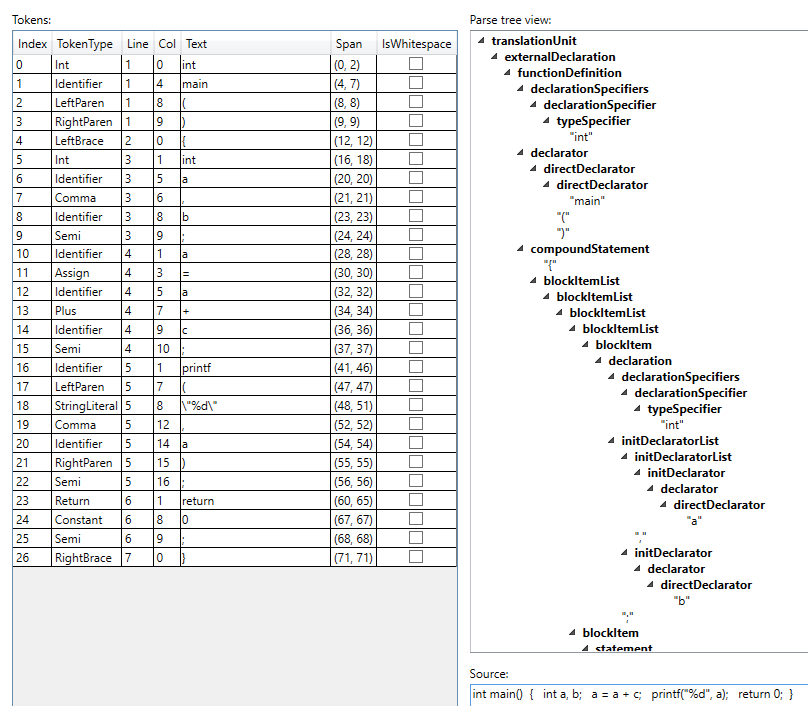
\includegraphics[width=\textwidth]{images/parse_tree.png}
}
\caption{Prikaz dela stabla parsiranja koje generiše parser kreiran od strane alata ANTLR4 \cite{ANTLR} za izvorni k\^od sa slike \ref{fig:CompilationProcessPrep}.}
\label{fig:CompilationProcessPars}
\end{figure}

Stablo parsiranja sadrži sve informacije potrebne u fazi parsiranja uključujući detalje korisne samo za parser prilikom provere ispunjenosti gramatičkih pravila. Sa druge strane, \emph{apstraktno sintaksičko stablo} sadrži samo sintaksičku strukturu u jednostavnijoj formi. Na slici \ref{fig:CompilationProcessPars1} se može videti koliko stablo parsiranja može biti kompleksno čak i za jednostavne aritmetičke izraze. Razlog kompleksnosti u ovom slučaju dolazi iz rekurzivnih pravila iz C11 gramatike. Parseru su sve ove informacije neophodne ali za naredne analize i proces prevođenja one nisu potrebne i zato se stablo parsiranja apstrahuje. Na primer, važna semantička odlika izraza \texttt{a+c} je da je to zbir vrednosti nekih promenljivih za razliku od pozicija delova ovog izraza u izvonom kodu. Na slici \ref{fig:ASTVariants} se mogu videti različita apstraktna sintaksička stabla za pomenuti izraz, ali takođe i za malo složenije izraze. Podrazumeva se, naravno, da je ulaz već tokenizovan. 

\begin{figure}[h!]
\centering
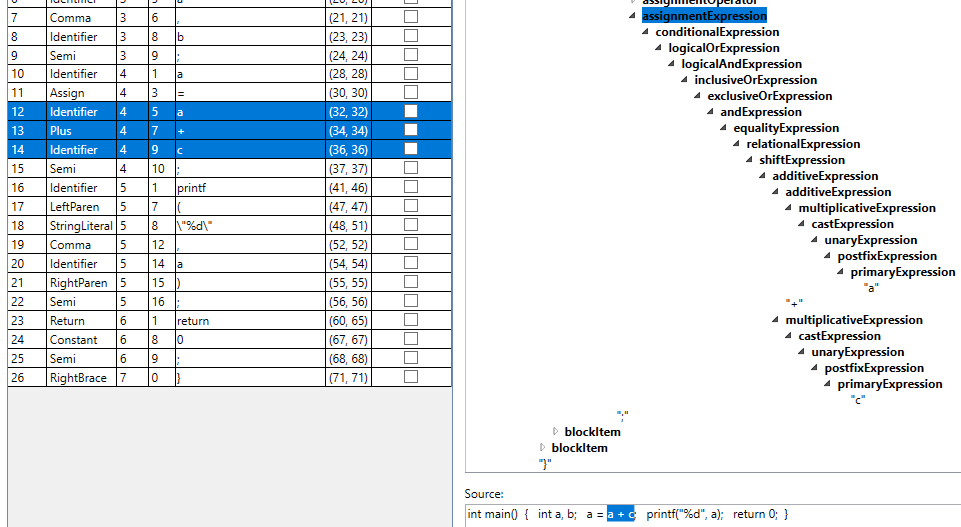
\includegraphics[scale=0.55]{images/parse_tree_expr.png}
\caption{Prikaz kompleksnosti stabla parsiranja za izraz 
\texttt{a+c} u C11 gramatici.} 
\label{fig:CompilationProcessPars1}
\end{figure}

\begin{figure}[h!]
\centering
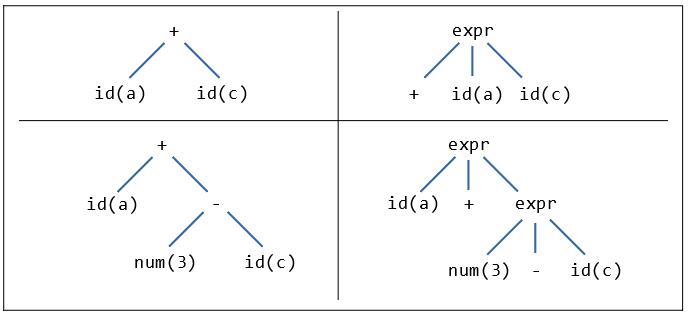
\includegraphics[scale=0.7]{images/ast.png}
\caption{AST varijante bez regularnosti (levo) i sa regularnošću (desno) za izraze \texttt{a+c} (gore) i \texttt{a+(3-c)} (dole).} 
\label{fig:ASTVariants}
\end{figure}

Uloga apstraktnog sintaksičkog stabla \cite{FormalSyntaxAndSemantics} je da pokaže semantiku strukture koda preko stabla. Kao što se vidi na slici \ref{fig:ASTVariants}, postoji određeni nivo slobode prilikom njegovog kreiranja. Generalno, \emph{terminalni simboli} --- simboli koji predstavljaju listove stabla parsera --- koji odgovaraju operatorima i naredbama se podižu naviše i postaju koreni podstabala, dok se njihovi operandi ostavljaju kao njihovi potomci u stablu. Desna stabla sa slike ne prate u potpunosti ovaj princip, ali se takođe koriste zbog regularnosti izraza --- ukoliko binarni izraz posmatramo kao apstrakciju, za implementaciju je lakše koristiti ovakav tip apstraktnih sintaksičkih stabala i stoga će biti korišćen kasnije u implementaciji opšte apstrakcije. Primetimo takođe da se u stablima za izraz \texttt{a+(3-c)} (dole) implicitno sačuvala informacija o prioritetu operacije oduzimanja u izrazu. Jasno je, dakle, da se računanje vrednosti aritmetičkih izraza onda vrši kretanjem od listova stabla ka korenu. Takođe, pošto je apstraktno sintaksičko stablo apstrakcija stabla parsiranja, više semantički ekvivalentnih izraza može imati isto apstraktno sintaksičko stablo ali različito stablo parsiranja; na primer, ako razmatramo izraz \texttt{(a+5)-x/2} i izraz \texttt{a+5-(x/2)}.

